\section{Problema I: Bactracking}

\subsection{Introducción}

Vamos a utilizar un algoritmo de backtraking que,es lo mas parecido a hacer fuerza bruta y recorrer todas las posibilidades
de pintar cada elemento. Es decir, cada elemento tiene tres formas diferentes de colorearse: Rojo, Azul o Sin Color.
de esta forma las combinaciones para un elemento esta determinado por 3 valores, luego para dos elemento las combinaciones son $3^2$
para k elementos $3^k$ por lo tanto la complejidad estará dada por $3^n$ donde n es la cantidad de elementos de la secuencia de números

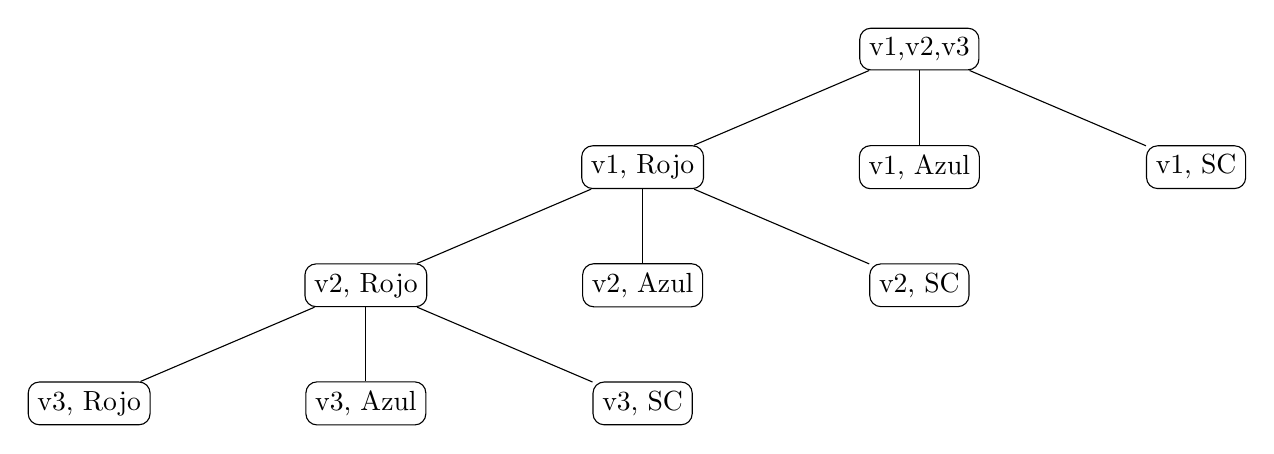
\begin{tikzpicture}[sibling distance=10em,
  every node/.style = {shape=rectangle, rounded corners,
    draw, align=center,
    top color=white, bottom color=white}]]
  \node {v1,v2,v3}
    child { node {v1, Rojo}
        child{ node {v2, Rojo}
            child{ node {v3, Rojo}}
            child{ node {v3, Azul}}
            child{ node {v3, SC}}}
        child{ node {v2, Azul}}
        child{ node {v2, SC}}}
    child { node {v1, Azul}}
    child { node {v1, SC}
 };
\end{tikzpicture}
\vspace*{5mm}

La solución está en las hojas del árbol, por lo tanto habrá que recorrer todo el árbol en peor caso para
encontrar la mejor solución.

\subsection{Resolución del problema y representación}
Para resolver este problema con backtracing, se iterará en toda la lista subsecuencias de tamaño 1 hasta el tamaño total de la secuencia
buscando la combinación máxima de elementos rojos y azules pintados. Para realizarlo presentaré el siguiente algoritmo.


Dicho  algoritmo tiene como representación dos vectores uno de enteros no negativos llamado elementos, otro de booleanos llamado validar y dos pilas una roja y otra azul con las siguientes características:
\begin{itemize}
    \item Los elementos de las pilas son las posiciones de los elementos de las secuencias.
    \item Una pila es estrictamente creciente y la otra decreciente.
    \item Las pilas son disyuntas entre si.
    \item Todos los elementos de las pilas están en elementos.
    \item Cuando un elemento ingresa a una pila, se asigna false a la posición de validar del elemento que ingreso.
    \item el vector validar me permite saber que elemento puedo agregar a la pila.
\end{itemize}

\subsection{Algoritmo}


El algoritmo consta de las siguientes funciones:
\subsubsection{Triviales}
\begin{itemize}

\item \underline{Establecer Validos:} \newline
 toma una pila y el vector validar, y establece el invariante para que cuando la otra función sea llamada no pueda
elegir los elementos que están en la pila máxima.
\item \underline{Maximizar:}\newline toma el tamaño de las dos pilas y devuelve el tamaño máximo,  por ultimo bastaría restar este valor al tamaño de entrada y se obtiene
la cantidad de libres.

\underline{Observación:} Cada función tiene otra idéntica modificando las guardas para encontrar el caso inverso por ejemplo la secuencia creciente tiene una decreciente
y mientras que rojos maximiza la secuencia creciente azules maximiza la decreciente ambas teniendo en cuenta de no pisar la otra.

\underline{secuCreciente} procesa todos los elementos de la lista desde dos posiciones cualesquiera del vector y agrega los que son validos o mayores.
\end{itemize}

\begin{algorithm}[H]
\caption{Backtracking}
  \begin{algorithmic}[1]
    \Procedure{secuCreciente}{\texttt{secu(int):} elementos,\texttt{secu(bool):}  validar,\texttt{pila(int):} Pila,\texttt{int} inicio,\texttt{int} fin }
    \State iterador $\gets$ inicio
    \State \While{ (iterador $<=$fin) }
      \If{tamaño(pila) $==$ 0}
        \State pila.push(iterador)
          \State validar[iterador]$ \gets $ false
      \State \Else
        \State \If{elementos[iterador]  $ > $ elementos[pila.top()] $\&\&$ validar[iterador]}
          \State pila.push(iterador)
          \State validar[iterador] $ \gets $ false
          \EndIf
        \State iterador $ ++ $
      \EndIf
   \EndWhile
\end{algorithmic}

\underline{Complejidad:} $\mathcal{O}(fin-inicio )$\newline
\underline{Justificación:} debido a que como máximo hace un recorrido lineal.
\end{algorithm}


\begin{algorithm}[H]
\caption{Backtracking}
\begin{algorithmic}[1]
  \Procedure{subSecuRojaMaxima}{\texttt{secu(int)} elementos,\texttt{secu(bool):} validar,\texttt{pila (int):} &PilaMaxima,\texttt{pila (int):} &Pila,\texttt{int} fin,\texttt{int} it,\texttt{int} n,\texttt{bool} notermine   }
    \State
    \State \While{ (\neg pila.vacia $\land$ notermine ) }
    \State \While{ (it $<$ fin $\land$ notermine ) }
    \State SecuCreciente(elementos,validar,pila,it,fin)
    \State \If {pilamaxima.size()$>$ fin}
	\State	pilaMaxima $\gets$ pila
	\EndIf
	    \State \If {pila.size())$==$ fin}
	\State	notermine $\gets$ false
	\Else
    \State it $\gets$ pila.top()+1
    \State  validar[pila.top()]= true
    \State   pila.pop()
    \EndIf
    \State \If{pila.size() $!= $0}
    \State it $\gets$ pila.top()$+$1
    \State validar[pila.top()] $\gets$ True
    \State pila.pop()
    \EndIf
    \EndWhile
    \EndWhile
\end{algorithmic}
\underline{Complejidad:} $\mathcal{O}(c^c$)
\end{algorithm}

\underline{Justificacion:} Siendo p = pila.size(), sea c = p + inicio - fin. Supongamos que de entrada hay una tira de elementos crecientes menos el ultimo, la pila pasa a tener tamaño c
Luego, cada vez que termina el ciclo quito el primer elemento y llamo a la función SecuCreciente que recorre los elementos hasta el final
De manera tal que, en cada iteración resto un elemento a la pila pero recorro uno mas en secuCreciente haciendo que en todas las iteraciones recorra todos los elementos por cada iteración.




\begin{algorithm}[H]
\caption{Backtracking}
\begin{algorithmic}[1]
  \Procedure{Rojos}{\texttt{secu(int):} elementos,\texttt{secu(bool):} validar,\texttt{pila(int):} &PilaMaxima,\texttt{int} inicio,\texttt{int} fin   }
    \State
    \State notermine $\gets$ true;
    \State \While{ (validar[j] $==$ false $\land$ j $<=$ fin ) }
    \State j++
    \EndWhile
    \State \If {j $>$ fin}
	\State	notermine $\gets$ false;
	\EndIf
    \State \While{j $<=$ fin )}
    \State pila.push(j)
    \State validar[j] $\gets$ false
    \State subSecuRojaMaxima(elementos,validar,pilaMaxima,pila,fin,it,notermine)
    \State j++
    \EndWhile
\end{algorithmic}
\underline{Complejidad:} $\mathcal{O}(k*c^c)$
\underline{Justificacion:} Es el costo de la operacion subSecuRojaMaxima llamada k veces, desde inicio a fin.
\end{algorithm}



\begin{algorithm}[H]
\caption{Backtracking}
\begin{algorithmic}[1]
  \Procedure{CantLibres}{\texttt{secu(int):} elementos,\texttt{secu(bool):} validar} $\to $ \texttt{int}
    \State fin $\gets$ elementos.size();
    \For {$i = 0; i < n; i{+}{+}$}
    \State j $\gets$ i;
    \State \While{ (j $<$ fin) }
    \State Rojos(elementos,validar,pilaRoja,i,j)
    \State EstablecerValidos(validar,pilaroja)
    \State Azul(elementos,validar,pilaAzul,0,j)
    \State EstablecerValidos(validar,pilaroja)
	\State	res $\gets$ minimo(pilaAzul,PilaRoja)
	\EndWhile
	\EndFor
\State return res
\end{algorithmic}
\underline{Complejidad:} $\mathcal{O}(n*c^c)$
\end{algorithm}
\underline{Justificacion:} Rojos y azules tienen la misma complejidad, Establecer validos es lineal por lo que queda acotado, nada mas que azul recorre el total de los elementos n veces teniendo una complejidad de $n^{n+1}$
\subsection{Experimentación}


Queremos demostrar que la complejidad de este algoritmo es exponencial, para ello vamos a tomar una secuencia de 40 números y mediremos el tiempo
de ejecución del programa partiendo de 2 elementos y sumando de a 2 sucesivamente hasta llegar a los 40.
\subsubsection {experimento 1}
Vamos a crear 3 secuencias de números y luego las vamos a comparar para ver cual de las tres tiene peor complejidad.
\begin{itemize}
\item Secuencia de todos los elementos iguales
\item Secuencia de numeros random
\item Secuencia de elementos decreciente (supuesto peor caso)
\end{itemize}

\begin{figure}[h]
    \centering
    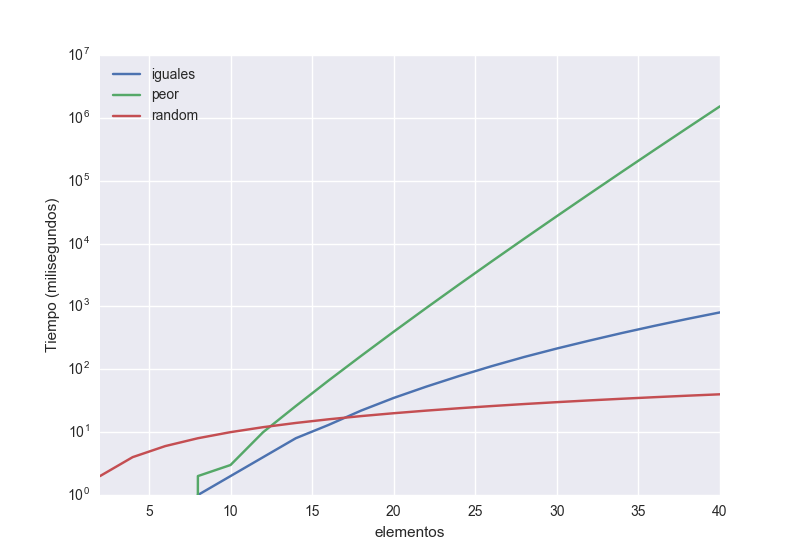
\includegraphics[width=0.55\textwidth]{figure_triple_1.png}
    \caption{Complejidad temporal}
    \label{fig:mesh1}
\end{figure}

Como podemos ver, en la figura 1 la que suponíamos peor caso,la de elementos decrecientes, es efectivamente así y se ve claramente como crece mas aceleradamente que el resto.
\subsubsection {experimento 2}
Una vez encontrada la secuencia de peor resultado, vamos a compararla contra una función exponencial y determinar el coeficiente de pearson entre dichas
funciones para determinar la correlación entre las curvas y luego comparar contra una función polinomial.
\begin{figure}[h]
    \centering
    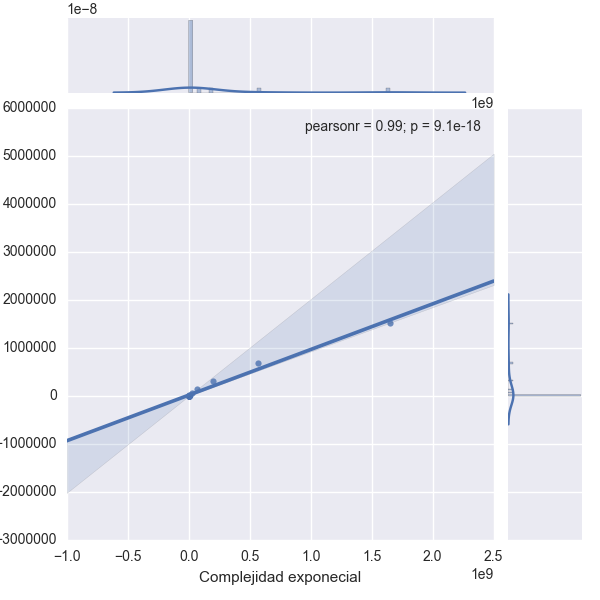
\includegraphics[width=0.38\textwidth]{figure_peor_1.png}
    \caption{Correlación}
    \label{fig:mesh1}
\end{figure}

\begin{figure}[h]
    \centering
    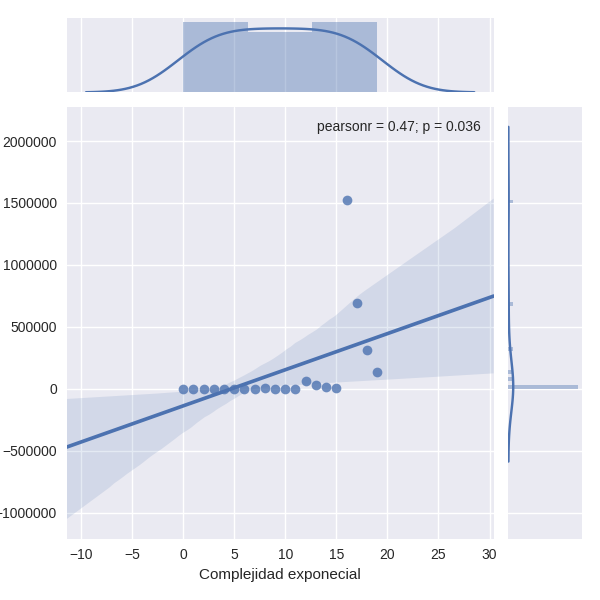
\includegraphics[width=0.38\textwidth]{pearson_ej1_2.png}
    \caption{Correlación}
    \label{fig:mesh1}
\end{figure}
Para determinar que la complejidad era exponencial, lo que hice fue  comparar esta secuencia de tiempos contra una funcion exponencial  $2^n$  y luego contra una función polinómica  $n^3$.Como resultado nos da un coeficiente de pearson de 0,99 para la función
exponencial  y un coeficiente de para la función polinómica lo que nos dice que nuestro programa se corresponde con la de una función exponencialy esto nos permite concluir que nuestro programa es exponencial, como se aprecia en la teoría.
